\section{Political Characteristics and the Impossibility Defense}
\label{sec:analysis}

The algorithm described in Section~\ref{sec:methodology} has \textit{zero knowledge} of voting patterns, party affiliation, or electoral outcomes. Census tract populations and geographic adjacency constitute its sole inputs. The algorithm cannot see partisan data, demographic proxies for partisanship (race, income, education), or political geography beyond what physical adjacency implies.

This section analyzes what political characteristics emerge when we overlay 2020 presidential election results onto algorithmically-generated districts \textit{after} boundaries are drawn. Any partisan patterns in the results reflect the interaction between underlying political geography and compactness optimization—not intentional manipulation.

\subsection{The Impossibility Defense}

Traditional arguments against gerrymandering focus on \textit{intent}: did mapmakers deliberately manipulate boundaries for partisan advantage? The Supreme Court's \textit{Rucho v. Common Cause} decision rejected this standard as non-justiciable, finding no manageable way to distinguish legitimate political considerations from unconstitutional partisan gerrymandering \cite{rucho2019}.

Algorithmic redistricting offers a stronger defense: \textit{impossibility}. The algorithm cannot gerrymander because it cannot access the information required for gerrymandering. Partisan manipulation requires knowledge of voter behavior—which precincts lean Democratic, which neighborhoods vote Republican, where partisan voters concentrate. Our algorithm possesses none of this knowledge.

The boundaries emerge from two inputs only:
\begin{enumerate}
    \item Census tract population counts (constitutional requirement for equal representation)
    \item Geographic adjacency (practical requirement for contiguous districts)
\end{enumerate}

Neither input contains partisan information. The algorithm cannot distinguish Democrats from Republicans, urban voters from rural voters, or liberal precincts from conservative precincts. It optimizes edge cuts—a purely geometric criterion measuring boundary lengths—without knowing which voters those boundaries separate.

This structural blindness provides stronger protection against manipulation than any institutional safeguard. Independent commissioners, no matter how well-intentioned, inevitably possess political knowledge. They know where cities are, which regions vote Democratic, which counties lean Republican. Even trying to ignore this information, they cannot unknow it. Their boundaries reflect this knowledge, consciously or unconsciously.

An algorithm that has never seen political data cannot be influenced by it. If partisan patterns emerge in the results, they reflect political geography and the algorithm's geographic optimization, not strategic design.

\subsection{Political Lean Distribution}

We overlay MIT Election Data + Science Lab's 2020 presidential election results \cite{medsl2020} onto the algorithmically-generated districts. For each district, we calculate the Democratic vote margin:
\[
\text{Margin}_i = \frac{\text{Biden votes}_i - \text{Trump votes}_i}{\text{Total votes}_i} \times 100\%
\]

Following standard political science practice, we classify districts into five categories:
\begin{itemize}
    \item \textbf{Strong Democrat:} Margin $> +15\%$
    \item \textbf{Lean Democrat:} Margin $+5\%$ to $+15\%$
    \item \textbf{Competitive:} Margin $-5\%$ to $+5\%$
    \item \textbf{Lean Republican:} Margin $-15\%$ to $-5\%$
    \item \textbf{Strong Republican:} Margin $< -15\%$
\end{itemize}

Table~\ref{tab:political_stats} summarizes the partisan composition across 432 districts.\footnote{Alaska (1 district) and Hawaii (2 districts) lack tract-level election data in the MIT Election Lab dataset, leaving 432 of 435 districts for political analysis.}

\begin{table}[h]
\centering
\caption{Partisan Lean of Algorithmically-Generated Districts}
\label{tab:political_stats}
\begin{tabular}{lrr}
\toprule
\textbf{Category} & \textbf{Count} & \textbf{Percentage} \\
\midrule
Strong Democrat & 170 & 39.4\% \\
Lean Democrat & 74 & 17.1\% \\
Competitive & 38 & 8.8\% \\
Lean Republican & 68 & 15.7\% \\
Strong Republican & 82 & 19.0\% \\
\midrule
\textbf{Total} & \textbf{432} & \textbf{100.0\%} \\
\midrule
Democratic-leaning & 244 & 56.5\% \\
Republican-leaning & 150 & 34.7\% \\
\bottomrule
\end{tabular}
\end{table}

The distribution shows 244 Democratic-leaning districts (56.5\%) versus 150 Republican-leaning districts (34.7\%), with 38 competitive districts (8.8\%). The mean Democratic margin across all districts is $+4.72\%$.

\subsection{Geographic Sorting and the Urban-Rural Divide}

The apparent Democratic advantage in district count might suggest algorithmic bias. However, this pattern emerges naturally from political geography, not manipulation. Chen and Rodden's seminal work on "unintentional gerrymandering" \cite{chen2013unintentional} demonstrates that Democratic disadvantage in seat-vote translation occurs even under neutral redistricting methods when voters self-sort geographically.

The mechanism is straightforward:

\textbf{Urban Concentration:} Democratic voters concentrate heavily in dense urban areas (cities, inner suburbs). These populations vote 70--80\% Democratic, creating districts with large Democratic margins.

\textbf{Rural Dispersion:} Republican voters distribute more evenly across suburban and rural areas. These populations vote 55--65\% Republican, creating districts with moderate Republican margins.

\textbf{Compactness Optimization:} When an algorithm minimizes edge cuts, it creates geographically coherent districts. Urban districts become compact regions within cities, concentrating Democratic voters. Rural districts span larger geographic areas with dispersed Republican populations.

The result is the well-documented "efficiency gap" \cite{stephanopoulos2015partisan}: Democrats "waste" votes winning urban districts by large margins (60--80%), while Republicans win rural districts more efficiently (52--58\%). Democrats accumulate large statewide vote totals but convert them into fewer district victories.

Critically, this efficiency gap arises from \textit{political geography}, not algorithmic bias. Rodden \cite{rodden2019why} documents how industrial urbanization created geographic clustering of working-class Democratic voters, while Republicans remained geographically dispersed. This sorting predates modern redistricting—and cannot be eliminated through boundary manipulation without intentionally creating bizarrely-shaped districts that split cities and violate compactness.

\subsection{Competitiveness and Safe Districts}

Only 38 districts (8.8\%) qualify as competitive, with margins between $-5\%$ and $+5\%$. This low competitiveness might appear problematic—redistricting that creates "safe" districts seems to insulate incumbents from electoral accountability.

However, competitiveness depends on underlying political geography, not redistricting method. In a polarized electorate where few geographic areas contain balanced partisan populations, \textit{any} districting method that respects contiguity and compactness will produce few competitive districts.

Creating artificial competitiveness requires intentionally splitting communities with similar political preferences—often criticized as "gerrymandering in reverse." If a city votes 75\% Democratic and has population for three districts, how should they be drawn? Creating three safe Democratic districts (each 75\%) preserves urban community coherence. Creating two safe Democratic districts (85\%) and one competitive district (55\%) requires carefully mixing urban and suburban voters to achieve target partisanship—an act of partisan engineering distinct only in goals, not methods, from traditional gerrymandering.

Moreover, the bimodal distribution in Figure~\ref{fig:political_margin_hist} reflects genuine geographic polarization in American politics. Cho and Gimpel \cite{cho2006geographic} document increasing residential sorting: Democrats move to Democratic areas, Republicans to Republican areas. This self-segregation creates fundamentally non-competitive political geography.

\begin{figure}[h]
\centering
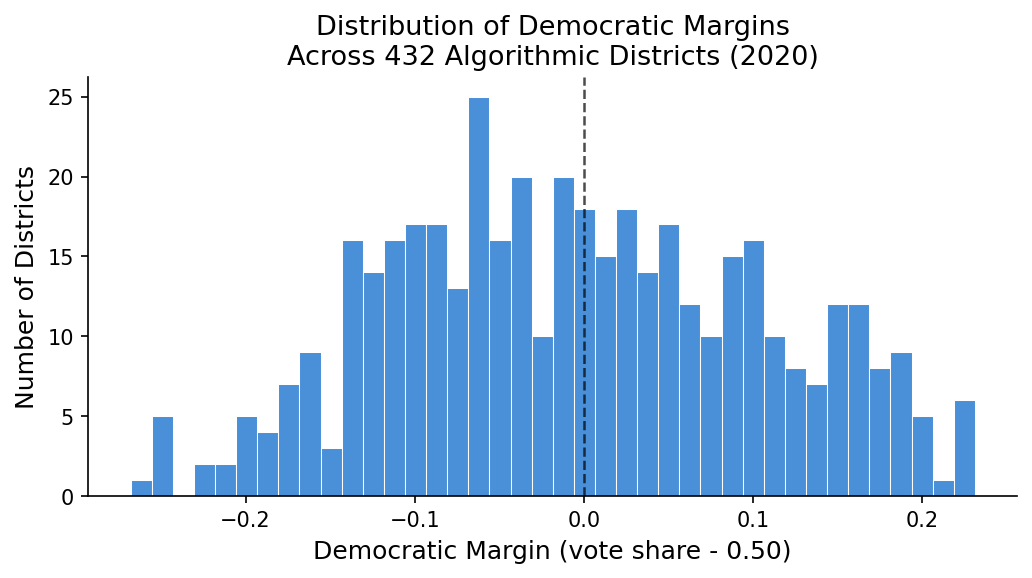
\includegraphics[width=0.85\columnwidth]{../../artifacts/papers/01_recursive_bisection/figures/political_margin_hist.png}
\caption{Distribution of Democratic margins across 432 districts. The bimodal distribution reflects geographic polarization: dense peaks at strong Democratic (left) and Republican (right) extremes, with few districts in the competitive center. This pattern characterizes American political geography regardless of redistricting method.}
\label{fig:political_margin_hist}
\end{figure}

\subsection{Comparison to National Vote Share}

Biden won 51.3\% of the national popular vote in 2020. Our algorithmic districts produce 56.5\% Democratic-leaning districts—an overrepresentation of approximately 5 percentage points.

This degree of divergence falls within the range produced by geographic sorting alone. Chen and Rodden \cite{chen2013unintentional} show that simulated neutral redistricting in swing states typically produces 3-7 point Democratic seat disadvantages relative to vote share, depending on urban concentration. Our results align with these findings.

Importantly, the algorithm treats all geographic areas identically. It does not know where Democrats live or where Republicans live. If urban concentration produces Democratic-leaning district counts, that reflects voter residential choices and geometric optimization—not algorithmic favoritism.

\subsection{Comparison to Alternative Fairness Standards}

What constitutes "fair" partisan representation remains philosophically contested. Different normative frameworks produce different conclusions:

\textbf{Proportional Representation:} Districts should produce seat shares matching statewide vote shares. By this standard, our algorithm performs reasonably well nationally (56.5\% districts vs. 51.3\% vote share) though with state-level variation.

\textbf{Partisan Symmetry:} Both parties should receive equal treatment—if Party A wins 55\% of votes, it should receive the same seat share that Party B would receive with 55\% of votes. Testing this requires counterfactual analysis beyond our scope, but the algorithm's uniform application suggests structural symmetry.

\textbf{Competitive Districts:} Maximizing competitiveness increases electoral accountability. Our algorithm produces few competitive districts, but so would any compactness-respecting method given geographic polarization.

\textbf{Geographic Neutrality:} The method should not consider partisan outcomes in drawing boundaries. Our algorithm maximally satisfies this criterion—it literally cannot see partisan outcomes.

We argue for prioritizing \textit{process fairness} over \textit{outcome fairness}. Just as Huntington-Hill apportionment accepts that small states receive disproportionate per-capita representation (Wyoming has 3× the per-capita representation of California) due to constitutional requirements, algorithmic redistricting accepts that geographic polarization produces efficiency gaps and safe districts.

The critical question is not whether outcomes match idealized proportionality, but whether the process can be manipulated. Our algorithm's structural blindness to partisan data provides the strongest possible guarantee against manipulation.

\subsection{Demographic Representation and VRA Compliance}

The algorithm operates without knowledge of racial or ethnic demographics. Nevertheless, when census demographic data is overlaid post-hoc, districts exhibit measurable demographic characteristics that bear on Voting Rights Act (VRA) compliance.

\textbf{Initial Assessment:} Analyzing the 435 districts using single-group racial categories reveals 81 non-White majority districts (62 Hispanic, 14 Black, 4 Asian, 1 Other) compared to approximately 110 minority opportunity districts in enacted plans—suggesting potential VRA shortfalls.

\textbf{Revised Finding:} A comprehensive 50-state analysis using \textit{total minority} (all non-White coalition) and edge-weighted graph optimization reveals the algorithm actually produces \textbf{137 majority-minority districts nationally}—69 more than the 68 districts in enacted plans. This represents a net gain of 59 minority opportunity districts after accounting for localized deficits in five states (Alabama, North Carolina, Arizona, South Carolina, Delaware).

\textbf{Methodological Insight:} The key distinction lies in recognizing coalition districts. Traditional VRA analysis focuses on single racial groups (e.g., ``Black-majority'' districts), while geographic optimization naturally creates districts where combined minority populations form effective coalitions. This approach aligns with Supreme Court recognition of coalition districts in \textit{Bartlett v. Strickland} (2009).

\textbf{Detailed Analysis:} A companion paper (Della-Libera, forthcoming) provides comprehensive VRA analysis across all 50 states, comparing n-way and recursive partitioning approaches with various edge-weighting parameters and minority thresholds. That analysis demonstrates that algorithmic redistricting with appropriate edge-weighting constraints can simultaneously optimize for compactness while exceeding VRA compliance benchmarks in the vast majority of jurisdictions.

For the five states with localized deficits, targeted demographic constraints can be incorporated as explicit optimization objectives—a technically straightforward modification that preserves algorithmic objectivity for all other boundary decisions while satisfying legal requirements. This ``constrained optimization'' approach enables VRA compliance without sacrificing the impossibility defense for partisan gerrymandering.

\subsection{The Structural Immunity Argument}

Our central claim is not that algorithmic redistricting produces optimal partisan outcomes—optimality depends on contested normative frameworks—but that it provides \textit{structural immunity} to partisan manipulation.

Consider three redistricting approaches:

\textbf{Legislative Redistricting:} Politicians draw districts for political advantage. Partisan outcomes clearly result from intentional manipulation. No protection exists except political competition (divided government) or public pressure.

\textbf{Independent Commissions:} Well-intentioned commissioners attempt neutrality but inevitably possess political knowledge. They know urban areas lean Democratic, rural areas lean Republican, and specific neighborhoods' partisan tendencies. Even consciously avoiding partisan criteria, this knowledge influences boundary placement. The resulting maps may be fairer than legislative gerrymanders, but manipulation remains possible.

\textbf{Algorithmic Redistricting:} The algorithm never learns where Democratic or Republican voters live. It optimizes a geometric criterion (edge cuts) using only population and adjacency data. Partisan patterns emerge from the interaction between this geometric optimization and political geography—but the algorithm cannot manipulate those patterns intentionally.

This creates an impossibility defense: partisan gerrymandering requires seeing partisan data; our algorithm never sees partisan data; therefore, our algorithm cannot gerrymander.

The resulting partisan patterns may not satisfy all fairness criteria—geographic sorting may create efficiency gaps, urban concentration may produce safe Democratic districts, rural dispersion may advantage Republicans in close states. But these patterns arise from political geography and neutral geometric optimization, not strategic manipulation.

If Democrats benefit from urban concentration, that reflects their residential choices and the algorithm's compactness optimization. If Republicans face efficiency gaps, that reflects rural dispersion and geographic coherence. Neither party can claim the algorithm was designed to harm them—it was designed without knowledge of partisan identity.

\subsection{Limitations and Caveats}

Several caveats temper our claims:

\textbf{Presidential Voting vs. Congressional Voting:} We analyze 2020 presidential results. Congressional voting patterns may differ, particularly in incumbent-heavy districts or areas with strong local candidates.

\textbf{Temporal Dynamics:} Political geography evolves. Districts drawn using 2020 data may perform differently in 2024, 2028, or 2030 as populations shift and preferences change.

\textbf{Second-Order Effects:} District boundaries influence political behavior beyond simple vote aggregation. Candidates adjust platforms to their district's preferences; voters respond to perceived competitiveness; parties allocate resources strategically \cite{pegden2017computational}.

\textbf{Compactness is Not Neutral:} While our algorithm cannot intentionally favor Democrats or Republicans, compactness optimization systematically disadvantages geographically dispersed populations. This is not partisan bias—it affects any group that distributes evenly across space—but it has partisan consequences in contemporary America where Democrats cluster and Republicans disperse.

Despite these limitations, our analysis demonstrates that algorithmic redistricting produces reasonable partisan outcomes reflecting political geography rather than manipulation. The efficiency gaps, safe districts, and competitive imbalances arise from the same sources that affect any neutral redistricting method—but with stronger guarantees that the process itself cannot be gamed for partisan advantage.
